
\begin{figure}
	\centering    
          \begin{tikzpicture}[->,>=stealth',shorten >=1pt,auto,node distance=.45cm,
  thick,main node/.style={observed}, hidden/.style={empty},background rectangle/.style={fill=olive!45}]
%every node/.style={scale=0.6}
 %nodes
\node[main node](1){$X_{1}$};
\node[main node, right=of 1](2){$X_{2}$};
\node[hidden, right=of 2](3){$...$};
\node[main node, right=of 3](4){$X_{N}$};
\node[main node, below right=of 2](5){$Y$};
\node[main node, above right=of 2](6){$Z$};
 \path[every node/.style={font=\tiny}]
    (1) edge (5)
    	(2) edge (5)
    (4) edge (5)
    (6) edge (1) edge (2) edge (4);
\end{tikzpicture}
        \caption{Confounded graph}
        \label{fig:parallel_confounded} 
\end{figure}


In this section we compare performance of our algorithms with the standard bandit algorithms on the confounded graph in figure \ref{fig:parallel_confounded}. All the variables are binary and the action space, $\calA$, consists of the set of single variable interventions $do(V_i = j)$. We choose this setting as it can be seen as a generalisation of the parallel bandit case and allows for factorizations that enable us to compute the exact reward distribution and interventional distributions for large $N$ (in general inference in graphical models is exponential in $N$). As before, we show the average regret over 10,000 simulations with error bars showing three standard errors. 

In figure \ref{fig:simple_vs_m_general} we fix $N$ and $T$ and $P(Z=1) = .4$. 

\eq{
P(X_i = 1|Z = 0) &= \begin{cases} 0 & \text{ if } i \in \set{1,...N_1} \\ .4 & \text{ otherwise } \end{cases}\\
P(X_i = 1|Z = 1) &= \begin{cases} 0 & \text{ if } i \in \set{1,...N_1} \\ .65 & \text{ otherwise } \end{cases}
}

As in the parellel bandit case, we let $Y$ depend only on $X_1$, $P(Y|do(X_1)=1) = \frac{1}{2} + \epsilon$ amd $P(Y|do(X_1=0)) = \frac{1}{2}-\epsilon'$, where $\epsilon' = \epsilon\frac{P(X_1=1)}{P(X_1=0)}$. We vary $N_1$ from 2 to $N$ to vary $m$. The values for the CPD's have been chosen such that the reward distribution is independent of $m$ and so that we can analytically calculate $\eta*$. This allows us to just show the dependence on $m$, removing the noise associated with different models producing selecting values for $\eta*$ with the same $m$ (and thus same worst case performance) but different performance for a given reward distribution. 

In figure \ref{fig:simple_vs_T_general} we fix the model and number of variables, $N$, and vary the horizon $T$. $P(Z)$ and $P(X|Z)$ are the same as for the previous experiment.  

In figure \ref{fig:simple_vs_T_misspecified} we exclude actions on $Z$ from the set of allowable actions to demonstrate how algorithm 1 can fail in the presence of a hidden confounding variable. Algorithm 1 incorrectly assumes $P(Y|do(X)) = P(Y|X)$ leading to biased estimates. To show the worst case outcome, where this bias results in Algorithm 1 asymptotically selecting a sub-optimal action, we need a slightly more complex CPD's. 

\eq{
P(X_i = 1|Z = 0) &= 
\begin{cases} 
.166 & \text{ if } i \in \set{1,...6} \\
.2 & \text{ if } i = 6 \\
.7 & \text { otherwise} 
 \end{cases}\\
 P(X_i = 1|Z = 1) &= 
\begin{cases} 
.166 & \text{ if } i \in \set{1,...6} \\
.8 & \text{ if } i = 6 \\
.3 & \text { otherwise} 
 \end{cases}\\
}

$Y$ depends only on $X_6$ and $X_N$. 
\eq {
P(Y|\boldsymbol{X}) = \begin{cases} 
a & \text{ if } X_6=0,X_N = 0 \\
b & \text{ if } X_6=0,X_N = 1 \\
c & \text{ if } X_6=1,X_N = 1 \\
d & \text{ if } X_6=1,X_N = 0 \\
\end{cases}
}


\begin{figure}[H]
    \begin{subfigure}[t]{0.3\textwidth}
		\centering    
    		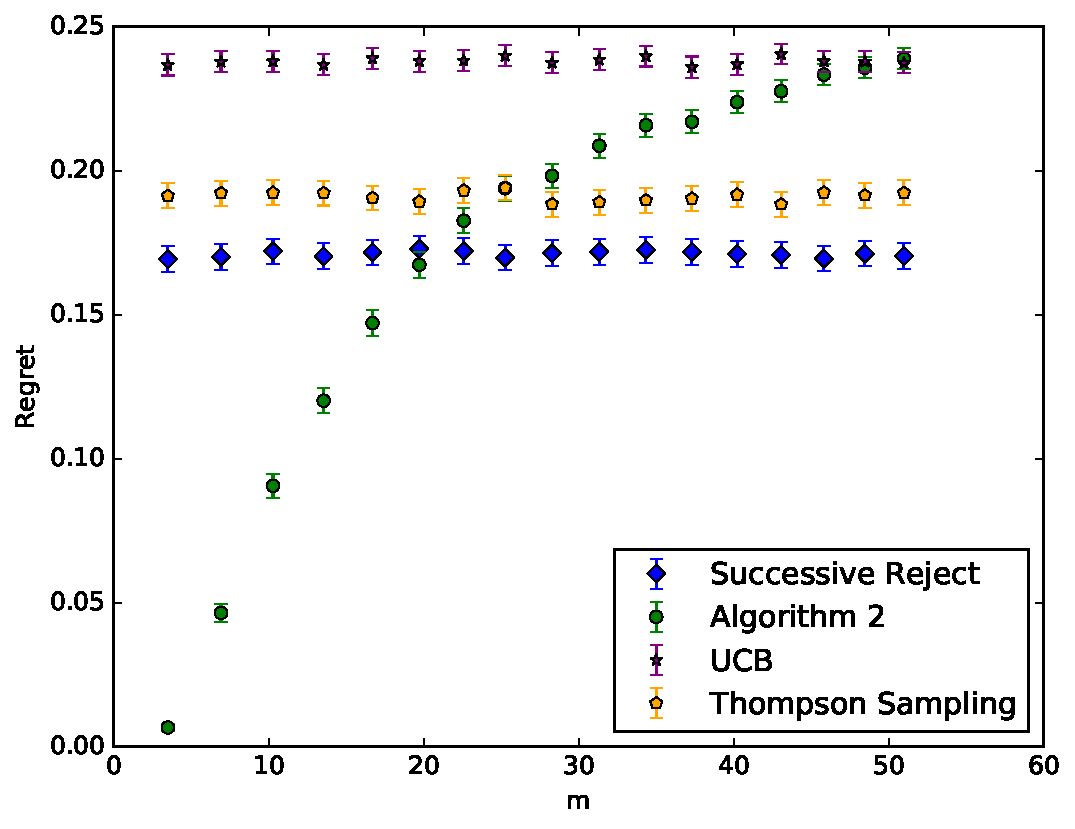
\includegraphics[width=\textwidth]{experiment4_20161012_1536.pdf}
    		\caption{Simple regret vs $m(\eta*)$ for fixed horizon $T=400$ and number of variables $N = 50$}
        \label{fig:simple_vs_m_general}
    \end{subfigure}\hfill
    \begin{subfigure}[t]{0.3\textwidth}
    		\centering
        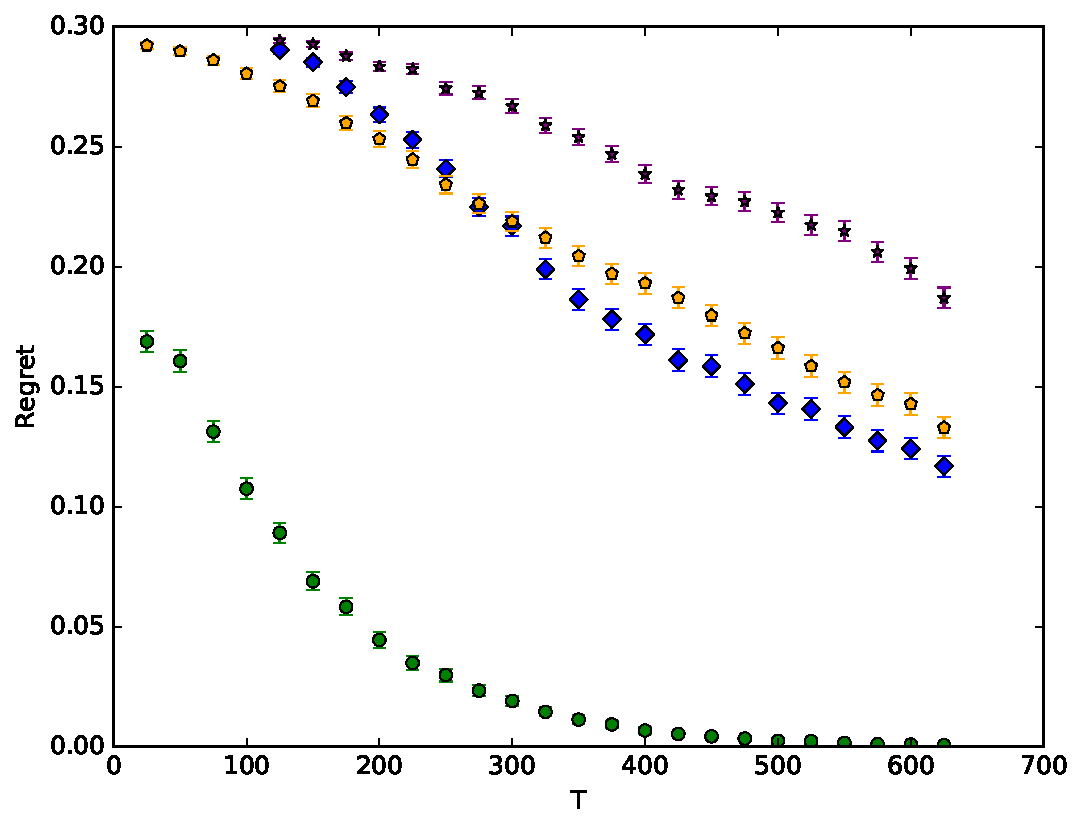
\includegraphics[width=\textwidth]{experiment7_20161012_1147.pdf}
    		\caption{Simple regret vs horizon, $T$, with $N = 50$ and $m(\eta*)=3.1$ }
        \label{fig:simple_vs_T_general}
    \end{subfigure}\hfill
    \begin{subfigure}[t]{0.3\textwidth}
    		\centering
    		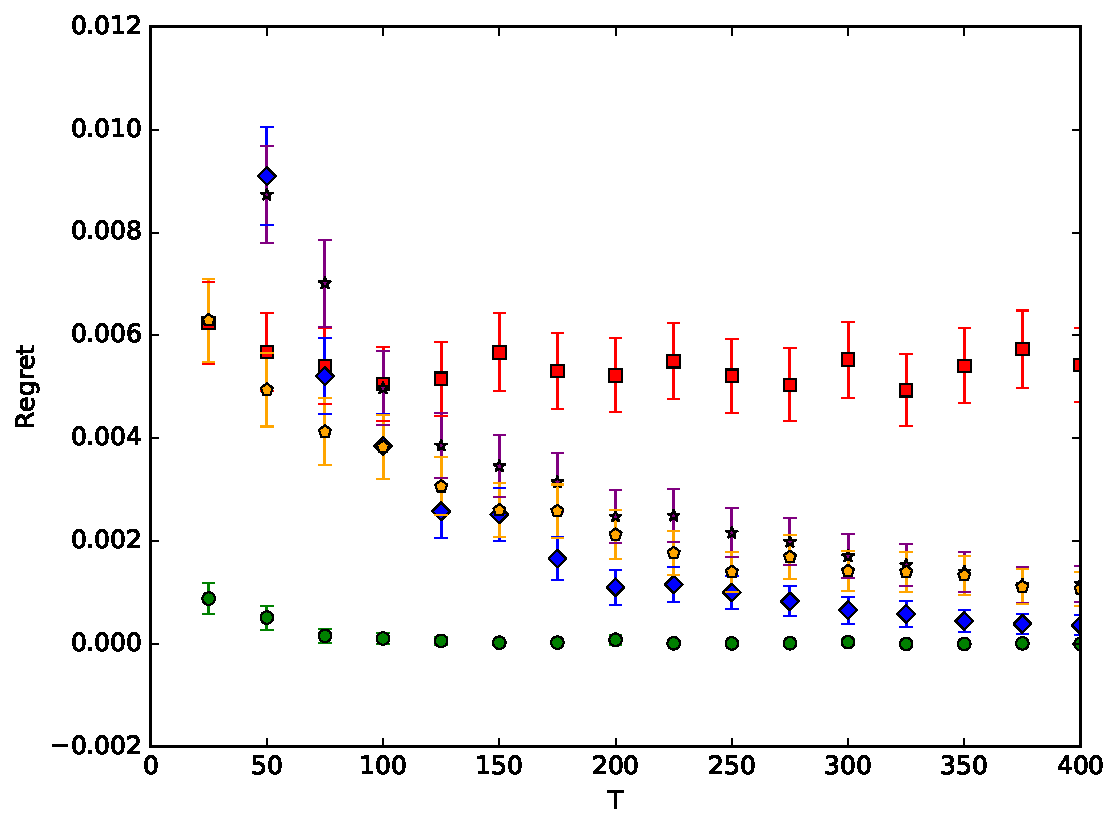
\includegraphics[width=\textwidth]{experiment5_20161014_0644.pdf}
    		\caption{Simple regret vs horizon, $T$, with $N = 20$, $m(\eta*)=4.4$ with no actions setting $Z$}
    		\label{fig:simple_vs_T_misspecified}
    \end{subfigure}
    \caption{Experimental results on the confounded graph}
    \label{fig:experiments}
\end{figure}



